\documentclass[a4paper]{article}

\usepackage{float}
\usepackage{graphicx}
\usepackage{tikz}
\usepackage{hyperref}
\usepackage[all]{hypcap}

\title{Computer vision lab 1}
\author{Xeryus Stokkel (s2332795)}

\begin{filecontents}{shear.data}
	#Shear	Matches
	0		98
	25		100
	50		91
	100		42
	200		3
	300		0
	400		0
\end{filecontents}

\begin{document}

\maketitle

\section{Exercise 1}

The SIFT implementation returns a key array of dimensions $1021 \times 128$. We know that a SIFT feature vector can either have a size of 128 or 160 elements, so from this we can see that there are 1021 keys in total. From \cite{lowe1999object} we know that the algorithm generates on the order of 1000 sift keys for a single image, so this is consistent with what has been found.

The keys found in the scene can be found in \autoref{fig:ex1keys}, as we can see most of the keys are on the objects that are sitting on the chair. most of the keys seem to be on the rice package while the book has the fewest amount of keys out of the three items at the top. When this is compared to Figure 3 from \cite{lowe1999object} it is the other way around, there the book has the most keys while the rice has the fewest.
\begin{figure}[h]
	\centering
	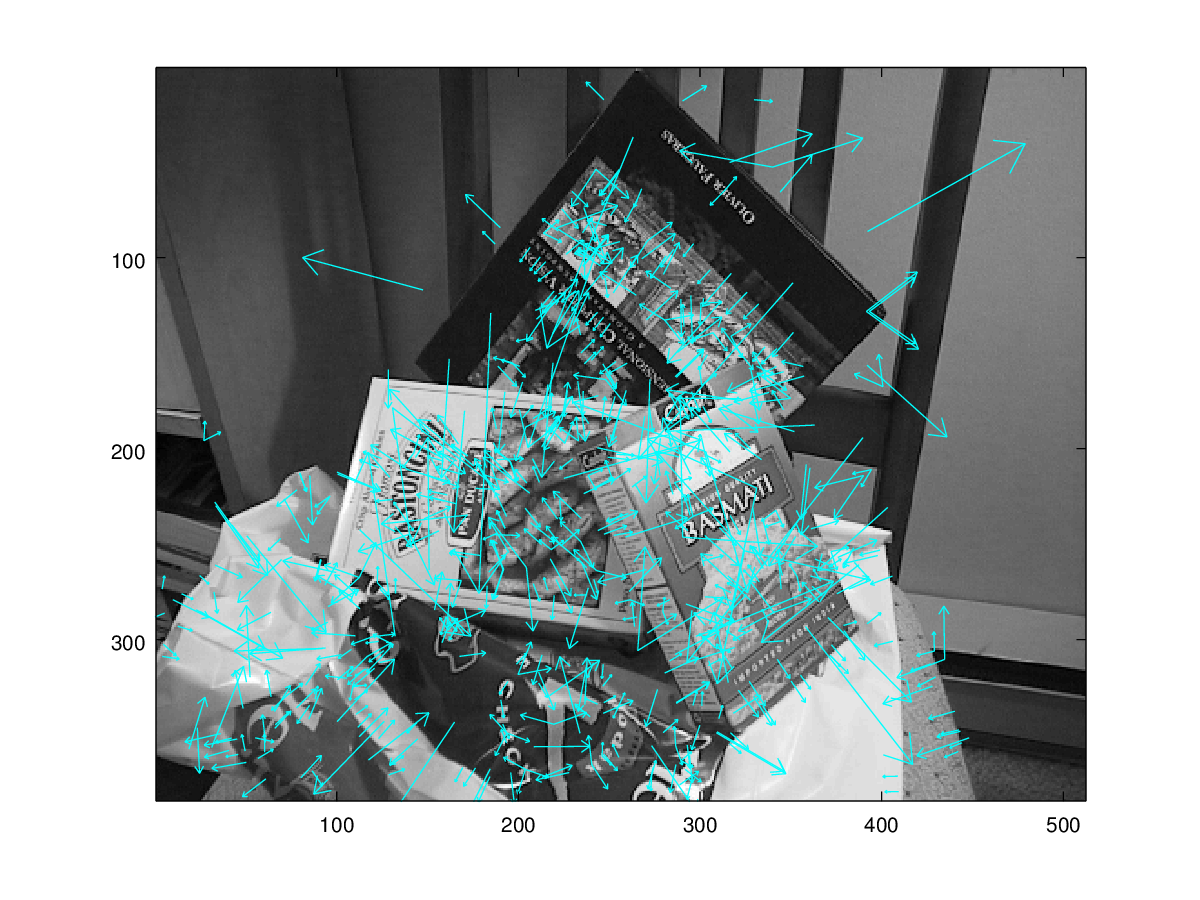
\includegraphics[width=.7\textwidth]{ex1keys}
	\label{fig:ex1keys}
	\caption{Location of the SIFT keys in scene.pgm}
\end{figure}

When matching the scene with the photo of the book cover we get 98 matches, these are shown in \autoref{fig:ex1match}. There are only two mismatches. The first is where a corner in the chair has been recognized as the corner of the book, this seems to be somewhat reasonable since they are both high contrast $90^\circ$ angle areas. The other mismatch is where a bit of the rice package got matched with one of the letters on the cover of the book. This is an odd match since there is just a random distribution of rice where the match occurs. Nevertheless, having only 2 mismatches in 98 total matches seems like a good result.

\begin{figure}[h]
	\centering
	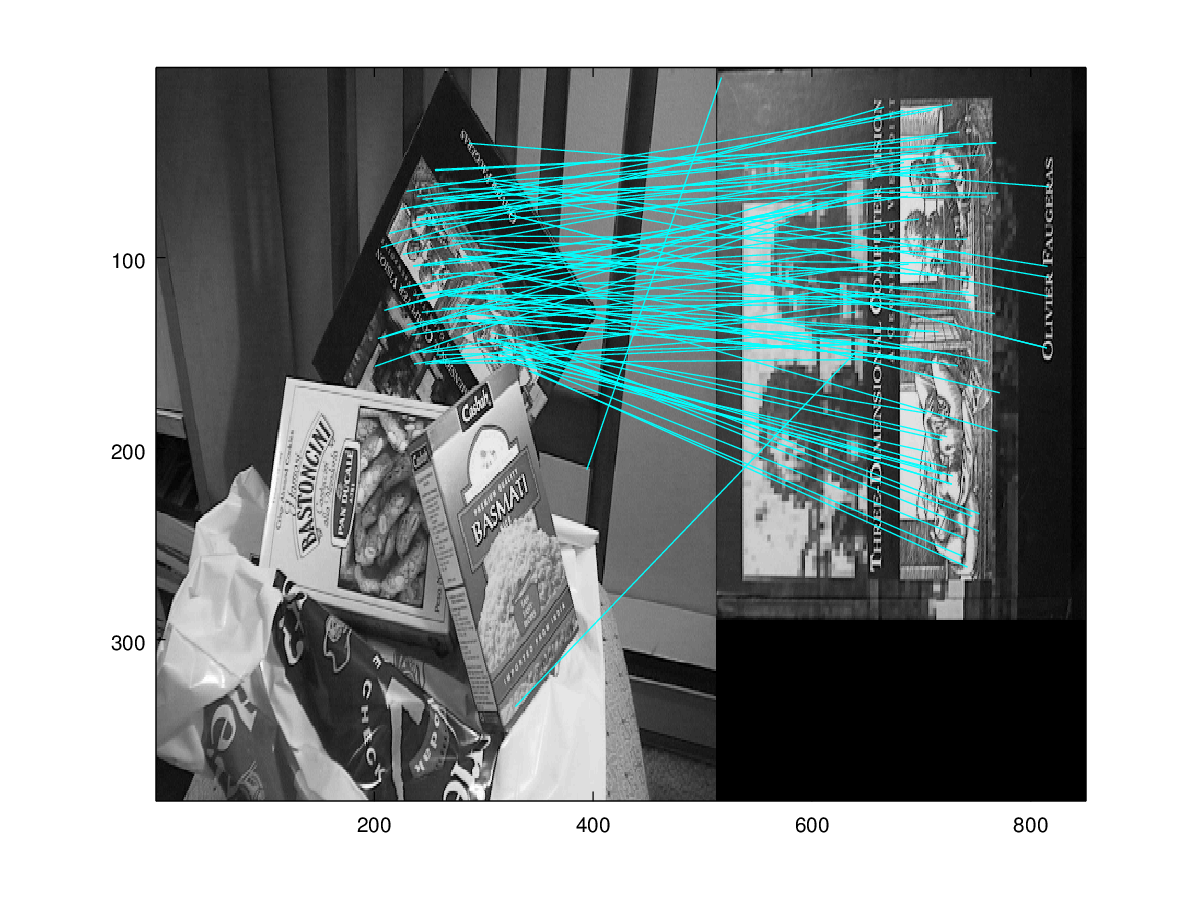
\includegraphics[width=.7\textwidth]{ex1match}
	\label{fig:ex1match}
	\caption{Matching locations in scene.pgm and book.pgm}
\end{figure}

Matching the scene with the Basmati package results in 34 matches, these are shown in \autoref{fig:ex1basmati}. There is only one mismatch in the image, this occurs on the border of the package that gets mismatched with part of the chair. Again both points in this mismatch have similar contrast.

\begin{figure}[h]
	\centering
	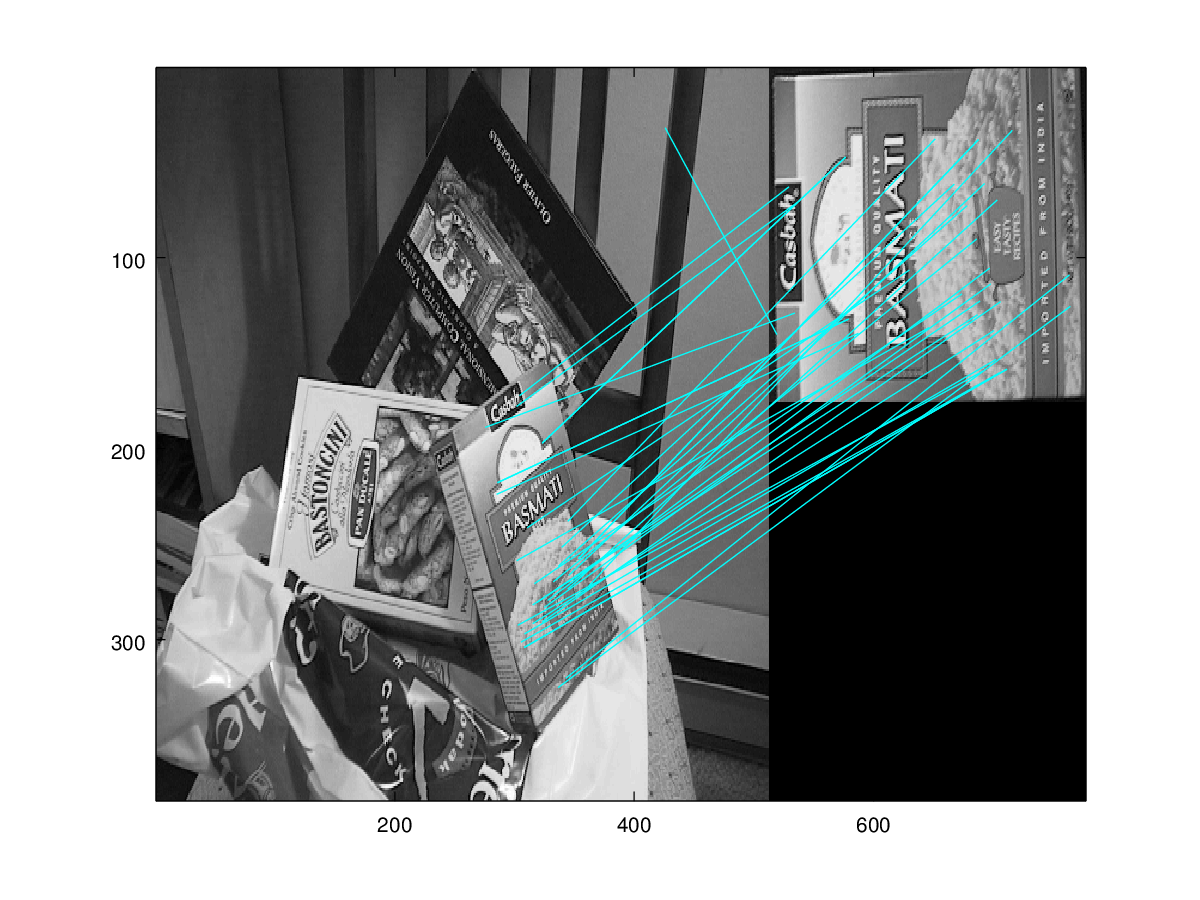
\includegraphics[width=.7\textwidth]{ex1basmati}
	\label{fig:ex1basmati}
	\caption{}
\end{figure}

The number of matches and errors per high and low resolution version of the street image are shown in \autoref{tbl:street}. The table clearly shows that the high resolution version has about 3 to 4 times as many matches but the number of errors also more strongly. So we get more information but a larger proportion is also in error. Some detail images also show errors where matches are within the target region but their exact location is incorrect, these have not been counted in \autoref{tbl:street}. This seems to mainly the case for the high resolution image. It thus seems that using a higher resolution doesn't improve the ability of SIFT to find matching features. On top of that processing the high resolution image also takes longer to process so from a processing time perspective the low resolution version is also better.

\begin{table}[h]
	\centering
	\caption{Number of matches per detail image vs. the low and high resolution version of the street.}
	\label{tbl:street}
	\begin{tabular}{l|r|r|r|r}
		& \multicolumn{2}{c|}{Small}& \multicolumn{2}{c}{Large} \\ \hline
		Detail 1 & 25 & 1 & 82  & 4 \\
		Detail 2 &  6 & 0 & 17  & 3 \\
		Detail 3 & 37 & 0 & 110 & 24 \\
		Detail 4 & 20 & 2 & 73  & 16 \\
		Detail 5 &  6 & 0 & 17  & 4
	\end{tabular}
\end{table}

\section{Exercise 2}
When trying to match the detail images against the indoor scene we find at most 2 matches. When the indoor details are compared against the low resolution outdoor scene we also find at most 2 matches. When we compare the indoor detail images against the high resolution we find at most 6 matches for the book while the other two detail images have 2 and 3 matches. This means that we can a threshold at 4 or higher and only one false positive would occur. A slightly more robust option is to have the number of matches be at least 1\% of the number of keypoints found in the image with the fewest keypoints.

\section{Exercise 3}
Matches for rotated images of the book are shown in \autoref{tbl:rotate}. The table shows that SIFT is rotation invariant. Both the number of matches and number of errors barely vary. Each orientation has around 100 matches.

\begin{table}[h]
	\centering
	\caption{Number of matches per rotated image of the book in the indoor scene.}
	\label{tbl:rotate}
	\begin{tabular}{l|r|r|r|r|r|r|r|r|r|r|r|r}
		Rotation & $0^\circ$ & $10^\circ$ & $20^\circ$ & $30^\circ$ & $40^\circ$ & $50^\circ$ & $60^\circ$ & $70^\circ$ & $80^\circ$ & $90^\circ$ & $180^\circ$ & $270^\circ$ \\ \hline
		Matches & 98 & 102 & 95 & 107 & 101 & 100 & 102 & 102 & 107 & 103 & 98 & 100 \\
		Errors  &  2 &   1 &  0 &   2 &   2 &   2 &   1 &   1 &   2 &   0 &  1 & 3 \\
	\end{tabular}
\end{table}

\section{Exercise 4}
The plot can be seen in \autoref{fig:shear}, and the exact data can be found in \autoref{tbl:shear}. We can see that a low amount of shear of up to 50 pixels does not influence the number of matches that much. More shear means that the number of matches sharply decreases so SIFT is only invariant to low amounts of shift but too much shift decreases its performance significantly.

\begin{table}[h]
	\centering
	\caption{Number of matches per sheared image in the indoor scene.}
	\label{tbl:shear}
	\begin{tabular}{l|r|r|r|r|r|r|r}
		Shear (pixels) & 0 & 25 & 50 & 100 & 200 & 300 & 400 \\ \hline
		Matches & 98 & 100 & 91 & 42 & 3 & 0 & 0
	\end{tabular}
\end{table}

\begin{figure}
	\centering
\begin{tikzpicture}[y=.05cm, x=.02cm]
	%axis
	\draw(0,0) -- coordinate (x axis mid) (425,0);
	\draw(0,0) -- coordinate (y axis mid) (0,100);
	%ticks
	\foreach \x in {0,50,...,400}
		\draw (\x,1pt) -- (\x,-3pt) node[anchor=north] {\x};
	\foreach \y in {0,10,...,100}
		\draw (1pt,\y) -- (-3pt,\y) node[anchor=east] {\y};
	%labels
	\node[below=0.8cm] at (x axis mid) {Shear (px)};
	\node[rotate=90, above=0.8cm] at (y axis mid) {Matches};
	
	\draw plot[] file {shear.data};
\end{tikzpicture}
	\caption{Plot of the number of matches vs. the shear of the detail image in pixels.}
	\label{fig:shear}
\end{figure}

\bibliographystyle{plain}
\bibliography{literature}

\end{document}